\label{chpt:discussion} % for referencing this chapter elsewhere, use \ref{chpt:label}
\lhead{\emph{Discussion}} % This is for the header on each page - perhaps a shortened title

With a reasonable sample of donor properties, and the resulting $\dot M$ and $\dot J$, I can now probe the data for correlations between these data.

First, however, I compare the mass loss rates of the $\dot M$ inferred from donor properties with the mass loss rates inferred from the white dwarf properties.
Figure~\ref{fig:massloss and AML:compare Mdot from donor and wd} plots the $\dot M$ from each method as a function of period -- note that this figure plots all the white dwarf based $\dot M$ regardless of if they were able to have donor based $\dot M$ found, so not every CV has two data points plotted.

It is immediately obvious that the white dwarf properties indicate a generally higher $\dot M$ than the donor properties, and do not follow the modelled donor tracks as the CV ages.
Conversely, the donor-derived $\dot M$ closely follows the `optimal' MESA model with gravitational braking amplified by a factor of $2.47$, even appearing to follow the period bounce regime though this is unlikely to be a real effect and is discussed later.
Interestingly, the white dwarf properties also suggest a much more \textit{consistent} mass loss rate across the CV population, with little scatter about $\sim 10^{-10} M_\odot~{\rm yr}^{-1}$ across the full period range.
% Correlations between the donor-derived $\dot M$ and various quantities are explored more thoroughly in \S\ref{sect:massloss and AML:mass loss rate correlations}.

This result is somewhat surprising given that we expect the donor properties to over-estimate $\dot M$ (\S\ref{sect:massloss and AML:systematic bias}), but Figure~\ref{fig:massloss and AML:compare Mdot from donor and wd} shows little indication of this.
Further, an explicit assumption in the white dwarf based $\dot M$ to be the total system $\dot M$ is that all material lost by the donor is accreted onto the white dwarf -- this is unlikely to be a robust assumption, as some material will be lost from the system without being accreted and would cause the white dwarf properties to indicate a lower system-wide $\dot M$ than reality.
Despite these factors, I observe generally \textit{higher} $\dot M$ with the white dwarf properties than with the donor.

The white dwarf indicating a higher mass loss rate may be a result of recent dwarf novae (i.e. periods of intense accretion onto the white dwarf), which cause the surface to temporarily heat up. After a dwarf nova has subsided, the white dwarf will take some time to readjust its temperature to the lower accretion rate, and for that period will appear to have an exaggerated accretion rate.
% Several of the CVs in this sample were identified for eclipse modelling follow-up \textit{explicitly} based on observations of recent dwarf nova outbursts.
OV Bootis \citep{Schwope2021} was observed to be $\sim 9000$K hotter than equilibrium 5 months after an outburst, and observations of GW Lib \citep{Szkody2016} show that the white dwarf is $\sim 3000$K hotter than equilibrium 8 years after an outburst.
Whilst such outburst could feasibly inflate the inferred $\dot M$, this would require a very recent outburst and would be extremely unlikely to affect every system in the sample. Further, the measurement uncertainty of the white dwarf $T_{\rm eff}$ in this sample is, on average, $\sim 2000$K - comparable to what one might reasonably expect from a recent dwarf nova. Assuming a recent nova heats a white dwarf by $5000$K, the apparent $\dot M$ would be increased only by $\log (\dot M, M_\odot\ {\rm yr}^{-1})\lesssim 0.2$ and should not radically alter the conclusions we can draw from these data.
At this time, the source of this discrepancy is unknown and more work is necessary to understand the tension between the two methods.

A system can be categorised as a period bouncer based on either the observed $M_{\rm donor}$, or the observed $\dot M$.
Despite this sample explicitly removing donors with masses typical of the post period minimum regime, three CVs have donor-inferred $\dot M$ that are consistent with the $\dot M$ of a period bounce CV: SDSS J0903, ASASSN-17fo, and OGLE82, though OGLE82 has an extremely uncertain $\dot M$ measurement of $\log (\dot M, M_\odot\ {\rm yr}^{-1}) = -11.686 \pm 1.078$.
This raises the question of an exceptionally poor understanding of the period minimum and period bounce regimes, but it must be noted that SDSS J0903 and ASASSN-17fo are peculiar systems for reasons previously mentioned in \S\ref{sect:modelling:donor mass loss rates}, and later revisited in \S\ref{sect:massloss and AML:measured angular momentum loss discussion}.
These two systems are instead more likely an artefact of systematic bias, discussed in \S\ref{sect:massloss and AML:systematic bias}, and only coincidentally lie on the period bounce donor track.

Hereafter, when values of $\dot M$ are used they are the values derived from the donor properties.

\begin{figure}
    \centering
    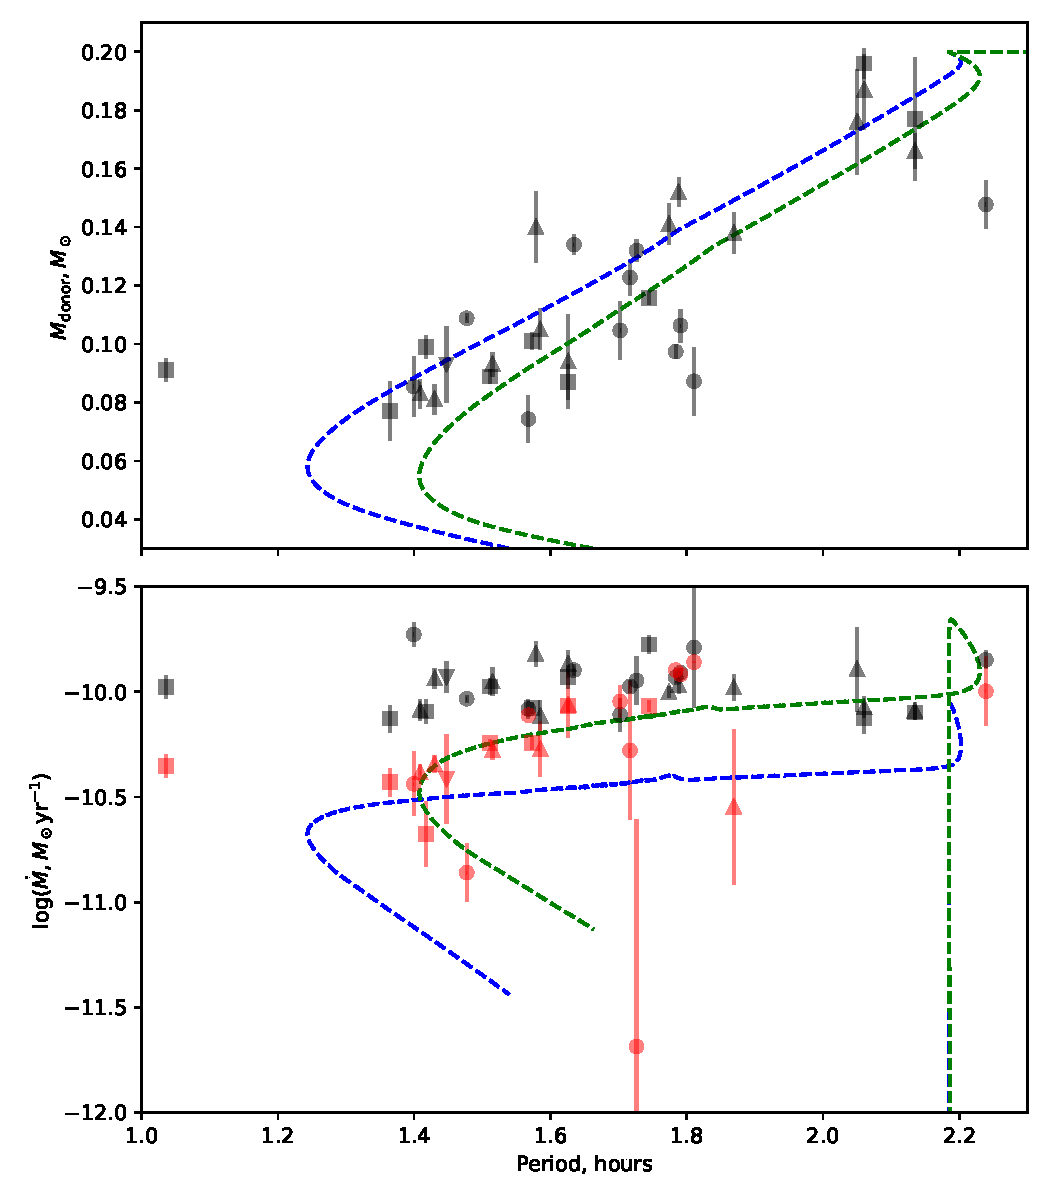
\includegraphics[width=\textwidth]{figures/results/Mdot/compare_mdot_from_donor_vs_wd_vs_period_withmasses.pdf}
    \caption{{\it Top}: Plotting the Period - $M_{\rm donor}$ relationship for the systems for which the white dwarf mass was determined.
    The MESA donor tracks are also plotted; the {\bf blue dashed line} shows the purely gravitational wave driven model, and the {\bf green dashed line} shows the model with gravitational braking amplified by a factor of $2.47$. The symbols denote the source of the data: {\bf circles} are the systems from Chapter~\ref{chpt:results:characterisation of 12 new CVs}, {\bf upright triangles} are data from \citet{McAllister2019}, {\bf squares} are from \citet{Savoury2011}, and the {\bf inverted triangle} is the supplementary system from \citet{mcallister2017b}.
        {\it Bottom}: Comparing the mass loss rates inferred from the donor properties ({\bf red data}) with those inferred from the white dwarf properties ({\bf black data}). Symbols are similar to the top panel.}
    \label{fig:massloss and AML:compare Mdot from donor and wd}
\end{figure}

\newpage
\section{Mass loss rate correlations}
\label{sect:massloss and AML:mass loss rate correlations}

Recall from the discussion in \S\ref{sect:introduction:magnetic braking} that, if the missing AML from CV models is rooted in residual magnetic braking, \textit{and these prescriptions for magnetism are accurate}, we would expect to see a correlation between $M_{\rm donor}$ and $\dot M$, and see no such correlation with $M_{\rm wd}$.
This is because both magnetic braking prescriptions considered are dependent on the Rossby number, a function of the rotational period, which itself is a function of donor mass for short period CVs. Note that the allowed mass range of the method used here forces us to omit period bouncer systems.
If, however, the CAML or eCAML model is correct, and the missing AML arises from white dwarf ejecta, (refer to \S\ref{sect:introduction:CAML}), we would expect a correlation between $M_{\rm wd}$ and $\dot M$, as in both cases there is a dependence of AML on the total system mass, which is dominated by $M_{\rm wd}$.
Of course, the two sources of extra AML are not mutually exclusive and may co-exist.

To probe for these correlations the $\chi^2$ test is insufficient, since both axes have significant uncertainty. The orthogonal distance between the line and data is minimised, similar to \S\ref{sect:12 new cvs:period excess}.
I report Pearson correlation coefficients and their associated $p$ values, computed based on the \textit{means} of the data, and do not consider the uncertainty in the measurements. Since uncertainty is ignored, these correlation coefficients are not technically correct, however, these values serve as a useful rough guide and are often easily corroborated by inspection of the relevant plots\footnote{Pearson correlation coefficients range from $-1$ (perfect negative correlation), to $+1$ (perfect positive correlation), with 0 indicating no correlation between the data. The $p$ value is the probability of the null hypothesis, i.e. that the data are uncorrelated, and values of $p < 0.05$ are generally accepted to indicate confidence in a correlation.}.

Figure~\ref{fig:massloss and AML:white dwarf mass vs Mdot fit} shows the data for $\dot M(M_{\rm wd})$, and Figure~\ref{fig:massloss and AML:donor mass vs Mdot fit} shows $\dot M(M_{\rm donor})$.
The correlation between $M_{\rm wd}$ and $\dot M$, is reasonably confident; ignoring errors, these data have a Pearson rank correlation coefficient of $-0.502$ and a $p$ value of $0.012$, indicating a high likelihood of a mild correlation. Fitting a straight line to these data supports this, finding a best-fit gradient that is $4.5\sigma$ from the null-hypothesis of 0.
However, no correlation is found between $\dot M$ and $M_{\rm donor}$. These data have a Pearson coefficient of $0.089$ with a $p$ value of $0.68$, and attempting to fit a straight line to the data results in an unconstrained gradient.

The relationship between $M_{\rm wd}$ and $\dot M$ has been previously observed, and justified theoretically by \citep{Pala2021}.
The luminosity of the white dwarf is related to both the radius and temperature, and the mass and mass loss rate,
\begin{equation}
    L \propto R^2_{\rm wd} T_{\rm eff}^4 \propto \dot M M_{\rm wd}^{0.4}
\end{equation}
By disregarding the weak mass relationship on the right side of this equation, we can approximate,
\begin{equation}
    \label{eqn:massloss and AML:white dwarf mass radius relationship to massloss}
    \dot M \propto R_{\rm wd}^2 T_{\rm eff}^4
\end{equation}
$R_{\rm wd}$ as a function of $M_{\rm wd}$ can be retrieved from the \citep{Bergeron1995} cooling tracks for a given $T_{\rm eff}$.
\citet{Pala2021} demonstrate that there is no observable correlation between white dwarf temperature, and white dwarf mass, so $T_{\rm eff}$ can be assumed to be the mean of the \citet{Pala2021} sample, $\sim 15000$K.
Note that whilst the gradient is weakly dependent on the chosen value of $T_{\rm eff}$, the difference within the range of reasonable CV temperatures ($\sim 5000 - 30000$K) is negligible.
The constant of proportionality is chosen by \citep{Pala2021} to reflect $\dot M = 7\times 10^{-10} M_\odot {\rm yr^{-1}}$ at $M_{\rm wd} = 0.8 M_\odot$, and I mirror this approach.

Thus, a prediction for approximate typical mass loss rates is found from the white dwarf sample in \citet{Pala2021}. Figure~13 from \citep{Pala2021} is reproduced in Figure~\ref{fig:modelling:pala2022 fig13}, and shows both the lack of correlation between $M_{\rm wd}$ and $T_{\rm eff}$, and the loose agreement between observations and Equation~\ref{eqn:massloss and AML:white dwarf mass radius relationship to massloss}.
I similarly compare my results with Equation~\ref{eqn:massloss and AML:white dwarf mass radius relationship to massloss} in Figure~\ref{fig:massloss and AML:white dwarf mass vs Mdot fit} alongside the best fit straight line, where it can be seen that this relationship agrees with the $3\sigma$ threshold of the best fit but appears less steep than the data suggests.
This illustrates that the mass loss rates I find from donor properties are loosely consistent with the recent findings of \citet{Pala2021}, despite the difference between the two methods seen in Figure~\ref{fig:massloss and AML:compare Mdot from donor and wd}.
\begin{figure}
    \centering
    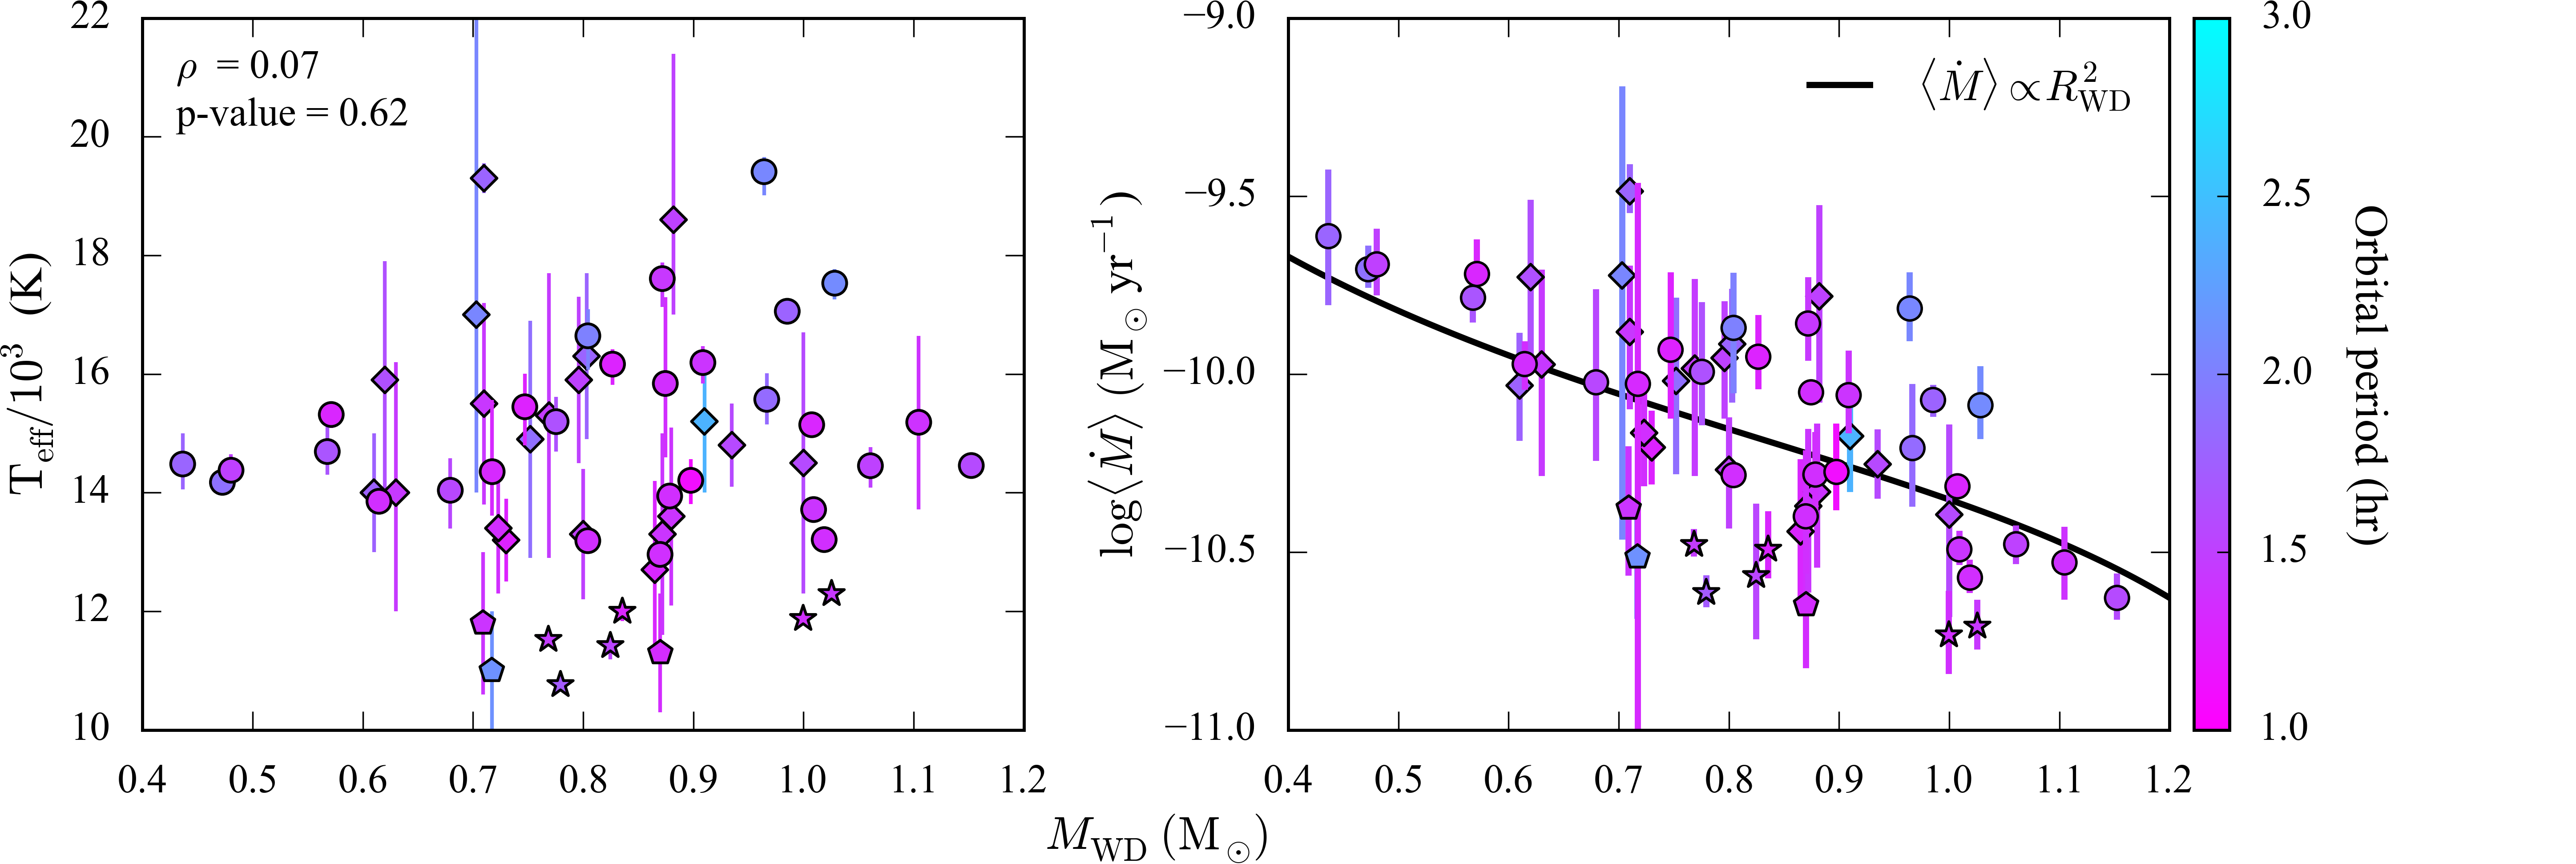
\includegraphics[width=\textwidth]{figures/modelling/pala_2022_fig13.png}
    \caption{Reproduced from \citet{Pala2021}, Figure~13. The subset of modelled systems, with $P < 3{\rm hr}$ are shown. {\bf Circles} and {\bf stars} are pre- and post-period bounce systems derived by \citet{Pala2021}, and {\bf diamonds} and {\bf pentagons} are pre- and post-period bounce systems taken from the literature. {\it Left}: The $T_{\rm eff}$ is plotted against $M_{\rm wd}$, and no correlation can be seen. {\it Right}: $\log \langle \dot M \rangle$ is plotted against $M_{\rm wd}$, though now the data are correlated along the white dwarf mass-radius relationship outlined by \citet{Pala2021}, $M_{\rm wd} \propto R_{\rm wd}^{2}$, shown by the {\bf black line}.}
    \label{fig:modelling:pala2022 fig13}
\end{figure}

Figure~\ref{fig:massloss and AML:compare Mdot from donor and wd} shows a reasonably tight agreement between the model MESA donor tracks and observed $\dot M$ and $P$.
One might expect to see this reflected in a plot of $M_{\rm donor}$ vs. $\dot M$ given the strong dependence of $M_{\rm donor}$ on $P$, but the agreement is more ambiguous with many data lying between the two model tracks.
This is likely related to the scatter about the models in Figure~\ref{fig:12 new cvs:donor model with eclipsers plotted}. As the mass-period relationship is synonymous with the mass-radius relationship, the scatter in Figure~\ref{fig:12 new cvs:donor model with eclipsers plotted} propagates forward.

Based on these results, it appears unlikely that residual magnetic braking (in the forms given in \S\ref{sect:introduction:magnetic braking}) is responsible for the excess AML in CVs, but still possible that the drag imposed by nova material is the cause.
However, there are a few factors to consider when deciding how convincing these findings are, beyond the important factors mentioned in \S\ref{sect:massloss and AML:systematic bias}.
The sample size is still small, only 24 systems, and the uncertainty in these measurements is significant.
More importantly, the parameter space between $0.12 M_\odot < M_{\rm donor} < 0.20 M_\odot$ is sparsely populated, and has particularly large uncertainty. This makes the search for correlation dominated by data in the narrow range of $0.08 M_\odot < M_{\rm donor} < 0.12 M_\odot$, and thus less robust; gathering more data for short period CVs with higher $M_{\rm donor}$ may yet reveal a correlation between donor mass and mass loss rate.
Also, the lack of correlation with $M_{\rm donor}$ may be a consequence of even the amplified `optimal' model $\dot M$ not varying by much across the donor mass range, a problem that may similarly be solved by expanding the available sample.
\begin{figure}
    \centering
    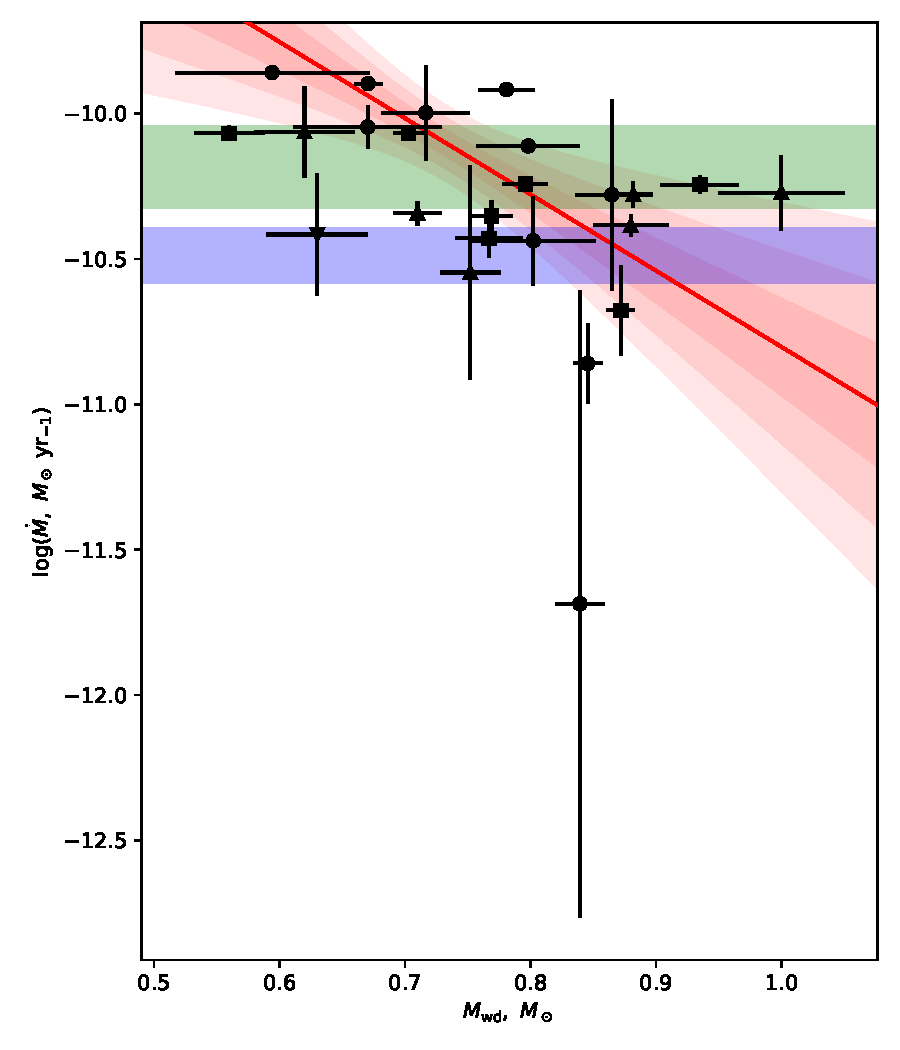
\includegraphics[width=\textwidth]{figures/results/Mdot/Mwd_Mdot.pdf}
    \caption{Showing the correlation between the white dwarf mass and mass loss rate. The {\bf black circles} are the systems from Chapter~\ref{chpt:results:characterisation of 12 new CVs} and have their system names labelled, {\bf gold upright triangles} are data from \citet{McAllister2019}, {\bf grey squares} are from \citet{Savoury2011}, and the {\bf brown inverted triangle} is the supplementary system from \citet{mcallister2017b}. The range of mass loss rates predicted by the `standard' and `optimal' MESA CV models are shown as the {\bf blue shaded region} and {\bf green shaded region}, respectively. The {\bf red line} shows the best fit to the data, with the {\bf shaded red region} showing the coverage of the uncertainty in the line parameters. The darkest region is $1\sigma$, the middle region is $2\sigma$, and the lightest region shows $3\sigma$. The best fit line has the form $\log ( \dot M,\ M_\odot\ {\rm yr}^{-1}) = (-2.62 \pm 0.60) (M_{\rm wd}, M_\odot) - (8.18 \pm 0.44)$. Also shown as the {\bf dashed green line} is the mass loss expected corresponding to a typical CV white dwarf $T_{\rm eff}$, following the relationship described in Equation~\ref{eqn:massloss and AML:white dwarf mass radius relationship to massloss}}
    \label{fig:massloss and AML:white dwarf mass vs Mdot fit}
\end{figure}
\begin{figure}
    \centering
    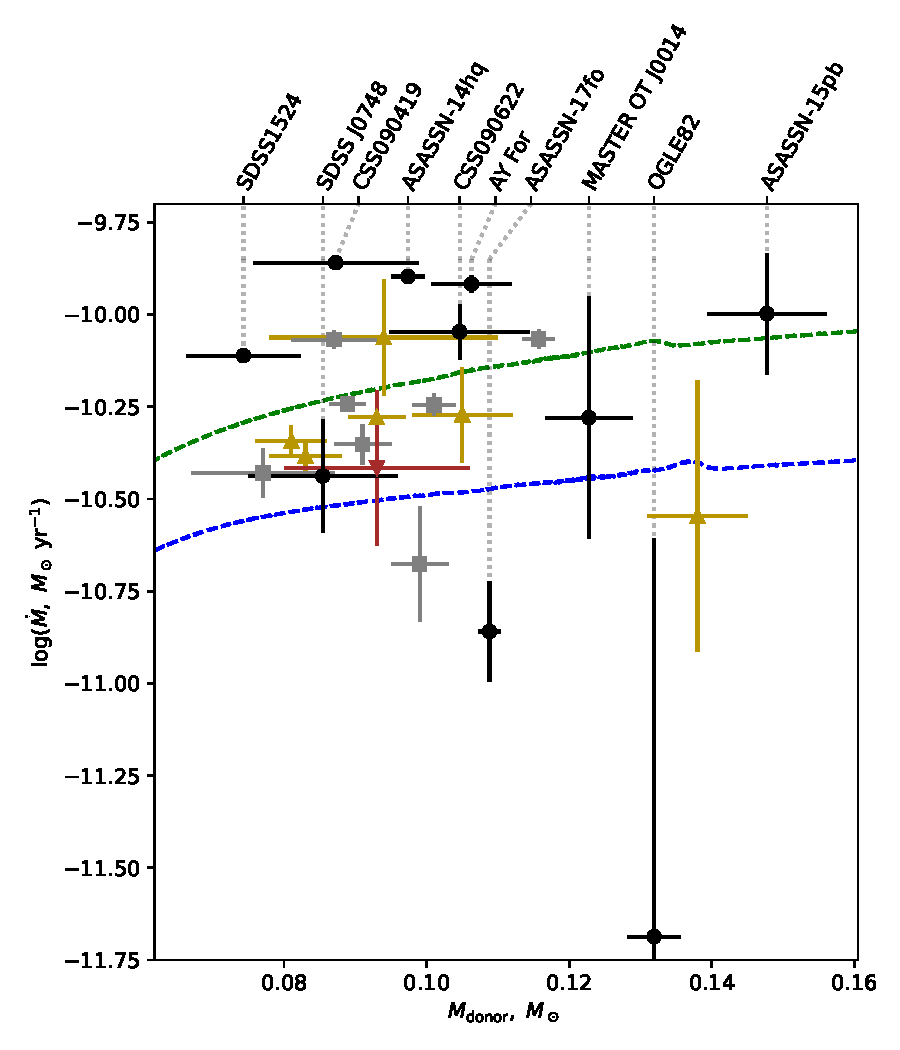
\includegraphics[width=\textwidth]{figures/results/Mdot/Mr_Mdot_nofit.pdf}
    \caption{Showing the donor masses and mass loss rates. Observations are styled similarly to Figure~\ref{fig:massloss and AML:white dwarf mass vs Mdot fit}. The {\bf dashed blue line} shows the value predicted by the `standard' MESA CV model, and the {\bf dashed green line} is the `optimal' MESA CV track.}
    \label{fig:massloss and AML:donor mass vs Mdot fit}
\end{figure}



\newpage
\section{Measured angular momentum loss}
\label{sect:massloss and AML:measured angular momentum loss discussion}

It is possible to more directly probe the AML of the CVs -- Equation~\ref{eqn:modelling:Jdot from Mdot} shows how the AML can be calculated from $M_{\rm wd},\ M_{\rm donor},\ \dot M$, and $a$.
Figures~\ref{fig:massloss and AML:donor mass vs Jdot fit}~and~\ref{fig:massloss and AML:white dwarf mass vs Jdot fit} show the $\dot J$ \textit{excess}, $\dot J_{\rm ex}$, which has had the $\dot J_{\rm GR}$ subtracted, against the two component masses.

Note that there are two peculiar systems in the sample, ASASSN-17fo and SDSS J0903, which were raised in \S\ref{sect:modelling:donor mass loss rates} and \S\ref{sect:massloss and AML:exploring massloss data} as having exceptionally low $\dot M$ and $\dot J$ estimates. Here, it can be seen that these systems appear to have sub-GR angular momentum loss, which is unphysical. Whilst there remains some doubt on the validity of these systems, they are still considered in the following analysis.

The $M_{\rm wd}$ and $\dot J_{\rm ex}$ data appear to be loosely correlated, with a Pearson correlation of $-0.514$ and a p-value of $0.010$. Fitting a straight line to the data finds $(\dot J_{\rm obs} - \dot J_{\rm MESA}) = (-8.3\pm1.6) \times 10^{27}(M_{\rm wd}, M_\odot) + (6.9\pm1.3)\times10^{27}~{\rm Joules}$.

However, similarly to the $\log (\dot M)$ data, there is no sign of correlation between $M_{\rm donor}$ and $\dot J_{\rm ex}$ -- these data have a correlation coefficient of $0.032$ and a p-value of $0.884$, strongly indicating that the data are uncorrelated and again suggesting that the magnetic braking prescriptions outlined in \S\ref{sect:introduction:magnetic braking} do not cause excess AML in short period CVs.

Based on period excess, three possibilities for the form of excess AML were suggested in \S\ref{sect:12 new cvs:period excess}: the excess AML declines in strength, but more slowly than gravitational losses; excess AML is roughly constant across the range of $M_{\rm donor}$ or $M_{\rm donor}$; or excess AML increases in strength towards lower $M_{\rm donor}$ or $M_{\rm wd}$.
The evidence suggests that excess AML appears to increase in strength towards lower $M_{\rm wd}$, and is uncorrelated with $M_{\rm donor}$.


\begin{figure}
    \centering
    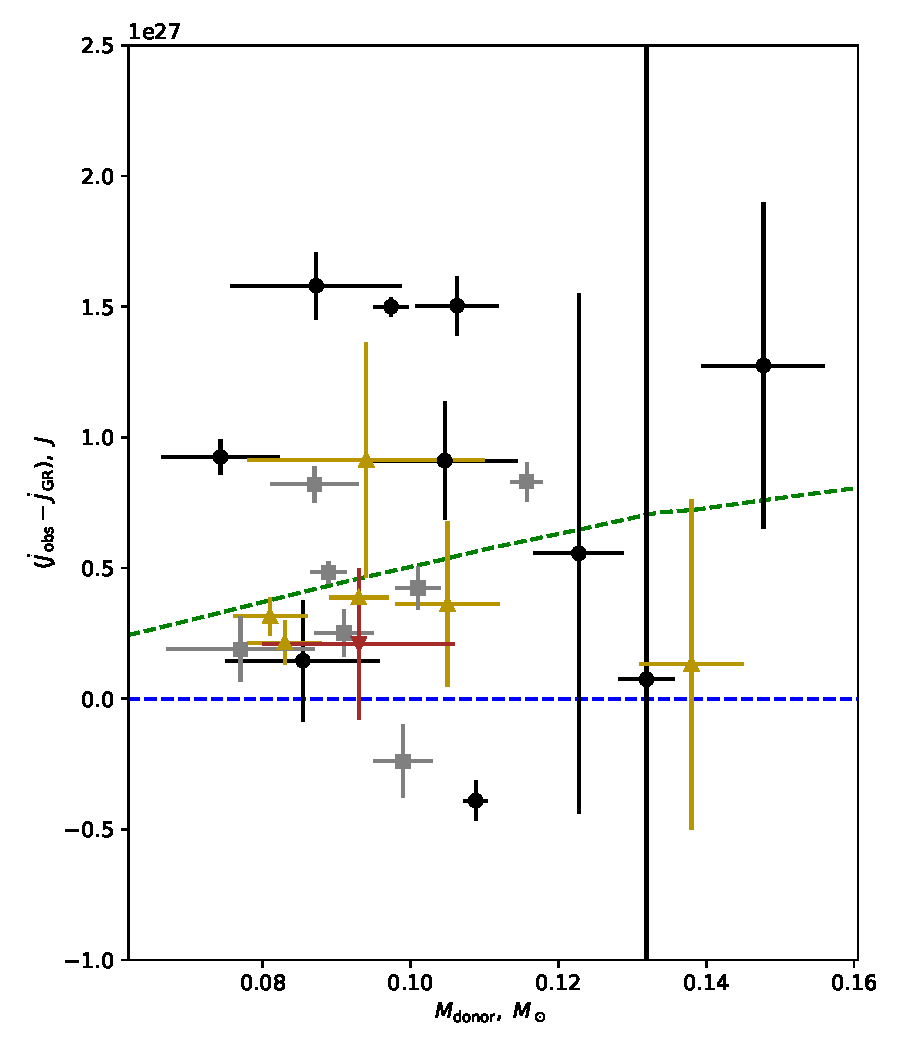
\includegraphics[width=\textwidth]{figures/results/Mdot/Mr_Jdot_nofit.pdf}
    \caption{Showing the correlation between the donor mass and angular momentum loss rate, $\dot J$. Observations are keyed similarly to Figure~\ref{fig:massloss and AML:white dwarf mass vs Mdot fit}, though here the {\bf dashed blue line} shows perfect agreement between observations and gravitational angular momentum loss. The {\bf dashed green line} shows the $2.47\times$ donor track.}
    \label{fig:massloss and AML:donor mass vs Jdot fit}
\end{figure}
\begin{figure}
    \centering
    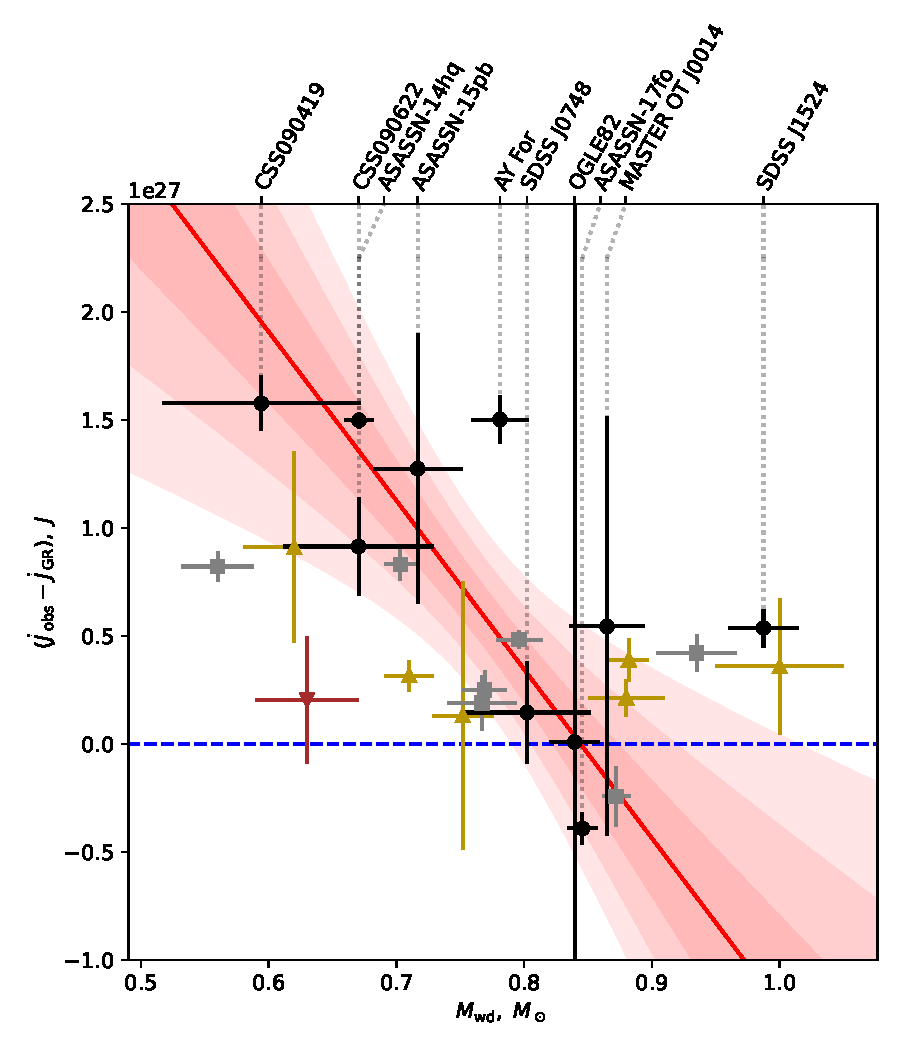
\includegraphics[width=\textwidth]{figures/results/Mdot/Mwd_Jdot_ex.pdf}
    \caption{Showing the correlation between the white dwarf mass and angular momentum loss rate, $\dot J$. Observations are keyed similarly to Figure~\ref{fig:massloss and AML:white dwarf mass vs Mdot fit}, and the best fit line has the form $(\dot J_{\rm obs} - \dot J_{\rm MESA}), J = (-8.3\pm1.6) \times 10^{27}(M_{\rm wd}, M_\odot) + (6.9\pm1.3)\times10^{27}$.}
    \label{fig:massloss and AML:white dwarf mass vs Jdot fit}
\end{figure}



\clearpage
\newpage
\section{A closer look at CAML}
Recall from \S\ref{sect:introduction:CAML} that under eCAML, the efficiency parameter $\nu$ is given by $C/M_{\rm wd}$, and typical values of $C$ are roughly chosen to be $0.3 - 0.4$ to reproduce the observed CV population distribution \citep{Schreiber2016}.
\begin{gather}
    \frac{\dot J_{ex}}{J} = \nu \frac{\dot M_{\rm donor}}{M_{\rm donor}} \label{eqn:caml general} \\
    \frac{\dot J_{ex}}{J} = C \frac{\dot M_{\rm donor}}{M_{\rm donor} M_{\rm wd}} \label{eqn:ecaml}
\end{gather}
% First, I assume that $\nu$ is a constant that can take any value, and fit this to the observations. Doing so finds a best-fit $\nu = 0.81\pm0.04$, shown in Figure~\ref{fig:massloss and AML:calibrating caml relationship}, though note that a constant $\nu$ is not a product of any CAML prescriptions.
$C$ can be fit to data, again minimising the orthogonal distance.
Doing so finds a best-fit $C = 0.58\pm0.02$, shown in Figure~\ref{fig:massloss and AML:calibrating ecaml relationship}, much higher than the previously estimated range of $0.3 - 0.4$, which is also plotted.
% The dynamically unstable region in $M_{\rm donor} vs. q$ space is expanded by the new value of $C$, and is shown in Figure~\ref{fig:massloss and AML:all cvs are dynamically unstable now}
Such a high value of $C$ is incompatible with the existence of short-period CVs, as this degree of CAML would render all short period systems dynamically unstable, which is clearly not the case. Whilst the sample size is small and the uncertainty in these measurements remains large, these preliminary results might be interpreted as a tension between the eCAML calibrated from population synthesis models by \citet{Schreiber2016}, and the calibration reported here.
However, such an interpretation is premature. As discussed in \S\ref{sect:massloss and AML:systematic bias}, the values reported here are subject to uncharacterised systematic bias, which likely causes an over-estimation of $\dot M$ and thus likely an over-estimation of $C$. Using the sample to calculate $C$ is therefore unwise, but the general trend present in these data remains promising. The measured $\dot J_{\rm ex} / J$ clearly lie on a straight line, $C$ is only a factor of 2 higher than expected, and the data are clearly strongly correlated with the quantities predicted by eCAML, implying that the theory is likely to be a good model of a future, more robust dataset.


% \begin{figure}
    %     \centering
    %     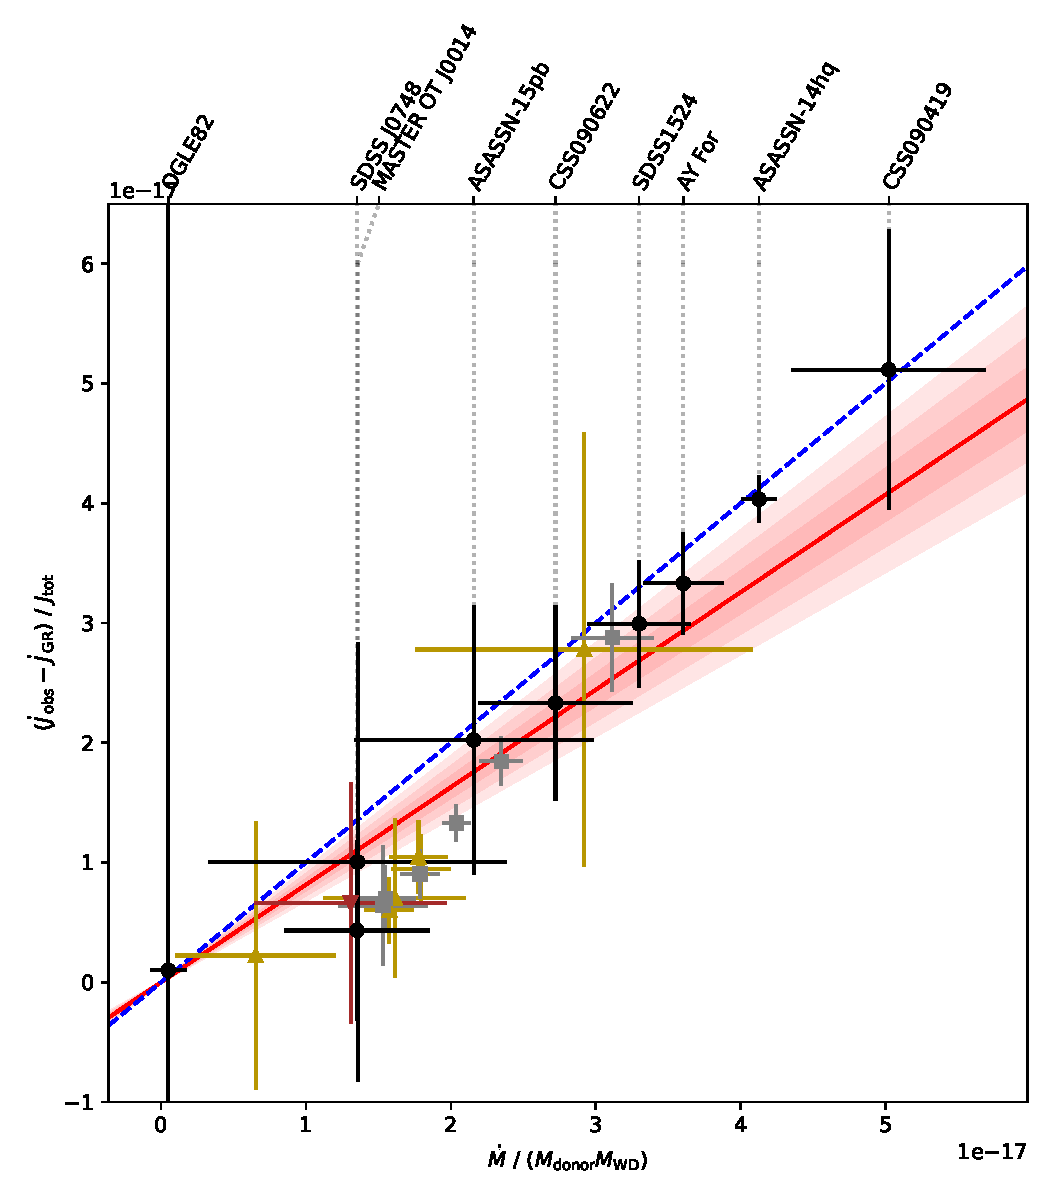
\includegraphics[width=\textwidth]{figures/results/Mdot/CAML_nu_with_intercept_fit.pdf}
    %     \caption{{\bf THIS WILL BE DELETED - X LABEL SHOULD ONLY HAVE MDONOR} Showing the observed quantities relevant to Equation~\ref{eqn:caml general} for short period CVs, based on donor properties. Symbols are as in Figure~\ref{fig:massloss and AML:white dwarf mass vs Mdot fit}, and the {\bf dashed blue line} shows the relationship for $\nu = 1$.}
%     \label{fig:massloss and AML:calibrating caml relationship}
% \end{figure}
\begin{figure}
    \centering
    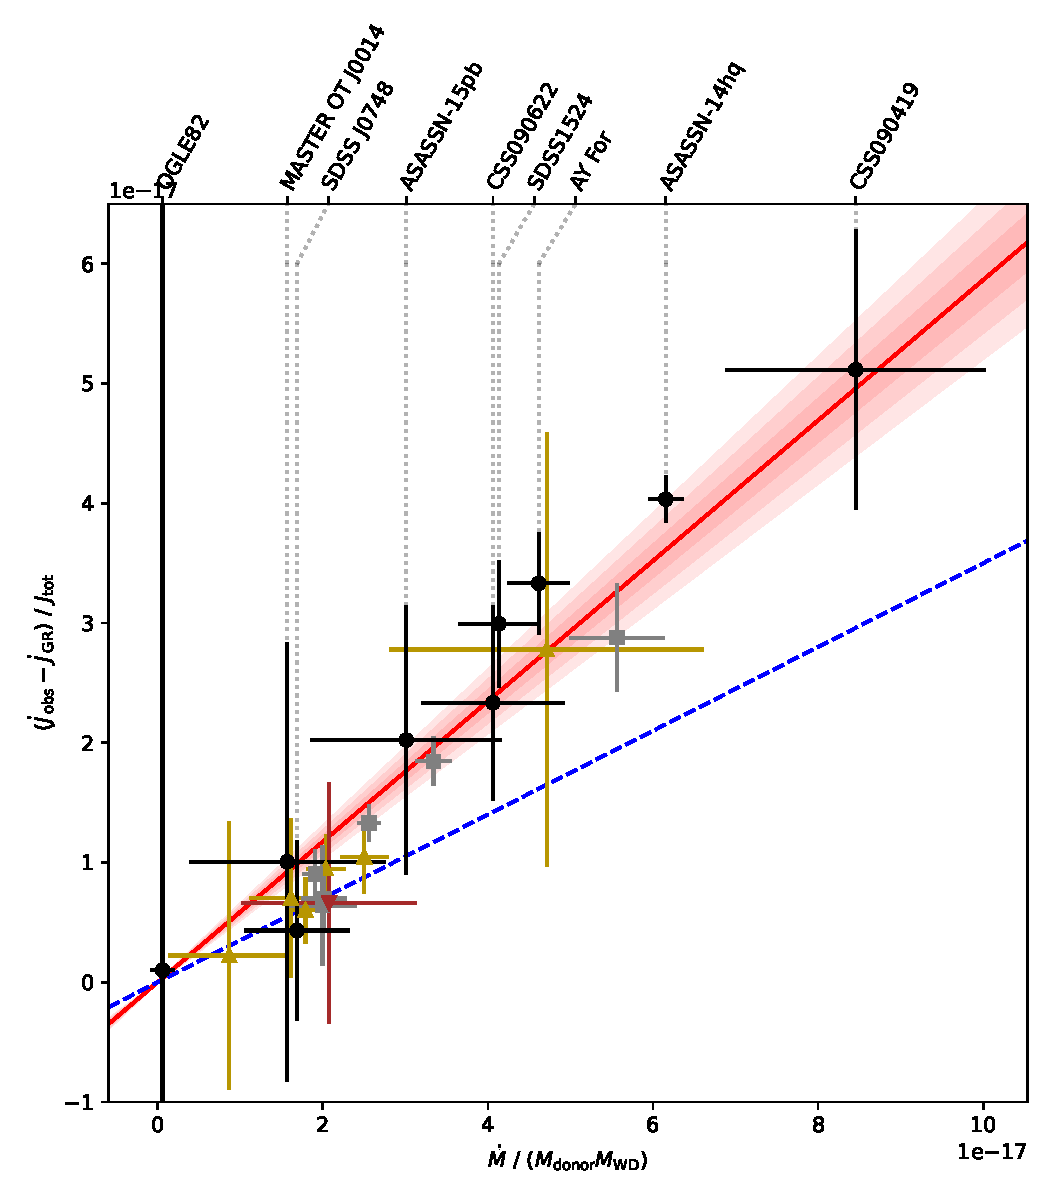
\includegraphics[width=\textwidth]{figures/results/Mdot/eCAML_nu_with_intercept_fit.pdf}
    \caption{Showing the observed quantities relevant to Equation~\ref{eqn:ecaml} and the best-fit value of $C$ for short period CVs, based on donor properties. Symbols are as in Figure~\ref{fig:massloss and AML:white dwarf mass vs Mdot fit}, and the {\bf dashed blue line} shows the relationship for $C = 0.35$.}
    \label{fig:massloss and AML:calibrating ecaml relationship}
\end{figure}
% \begin{figure}
%     \centering
%     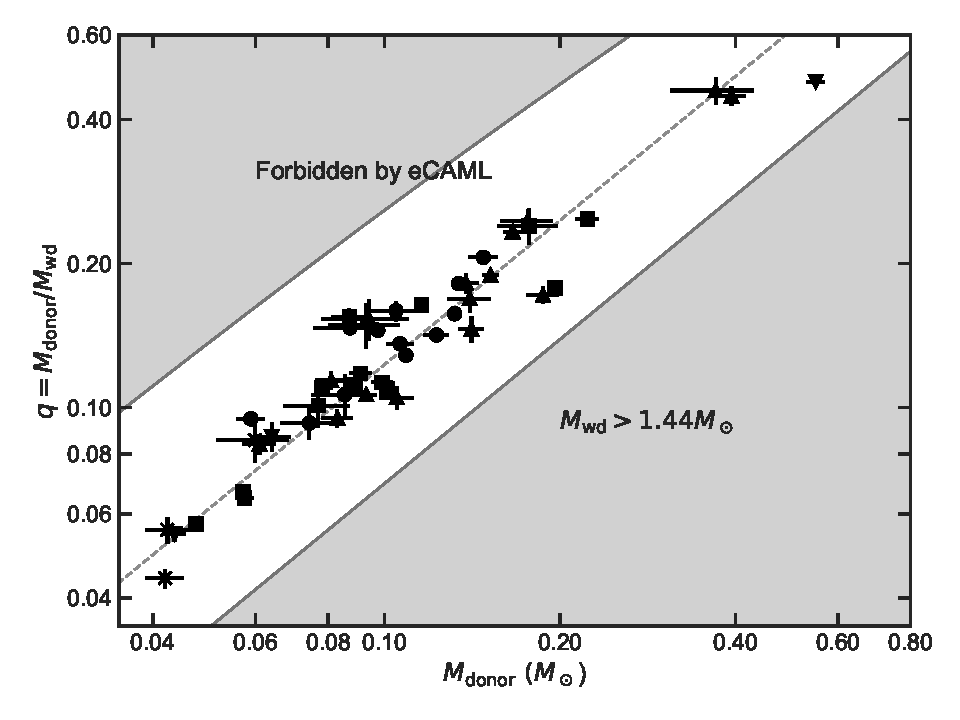
\includegraphics[width=\textwidth]{figures/results/Mdot/ecaml_nointercept.pdf}
%     \caption{Showing the allowed $q$ - $M_{\rm donor}$ combinations, under the new calibration of eCAML. Grey regions are forbidden - the upper region is dynamically unstable under eCAML, and the lower region has a white dwarf massive enough to trigger a supernova. Data are plotted with the same symbology as Figure~\ref{fig:massloss and AML:white dwarf mass vs Mdot fit}, and the dashed black line corresponds to $M_{\rm wd} = 0.82 M_\odot$.}
%     \label{fig:massloss and AML:all cvs are dynamically unstable now}
% \end{figure}

A further comparison with the previous eCAML calibration is possible by calculating $\nu$ for each system.
The $\nu$ values are plotted as a function of white dwarf mass in Figure~\ref{fig:massloss and AML:calculated nu for all short period CVs}, alongside the predicted $\nu$ for eCAML, $\nu = C / M_{\rm wd}$.
As the uncertainties in both $\dot J/J_{\rm tot}$ and $\dot M / M_{\rm donor}$ are large, the uncertainty in the calculated $\nu$ is too large to draw confident conclusions; however, it still provides a useful indication of what we might expect from future results.
Whilst some data are consistent with the \citet{Schreiber2016} eCAML calibration, it appears to generally under-estimate the mass loss from short period CVs with a significant portion of the data consistent with $\nu \sim 0.9$\todo{On this plot, add a line for $C = 0.58$}.
\begin{figure}
    \centering
    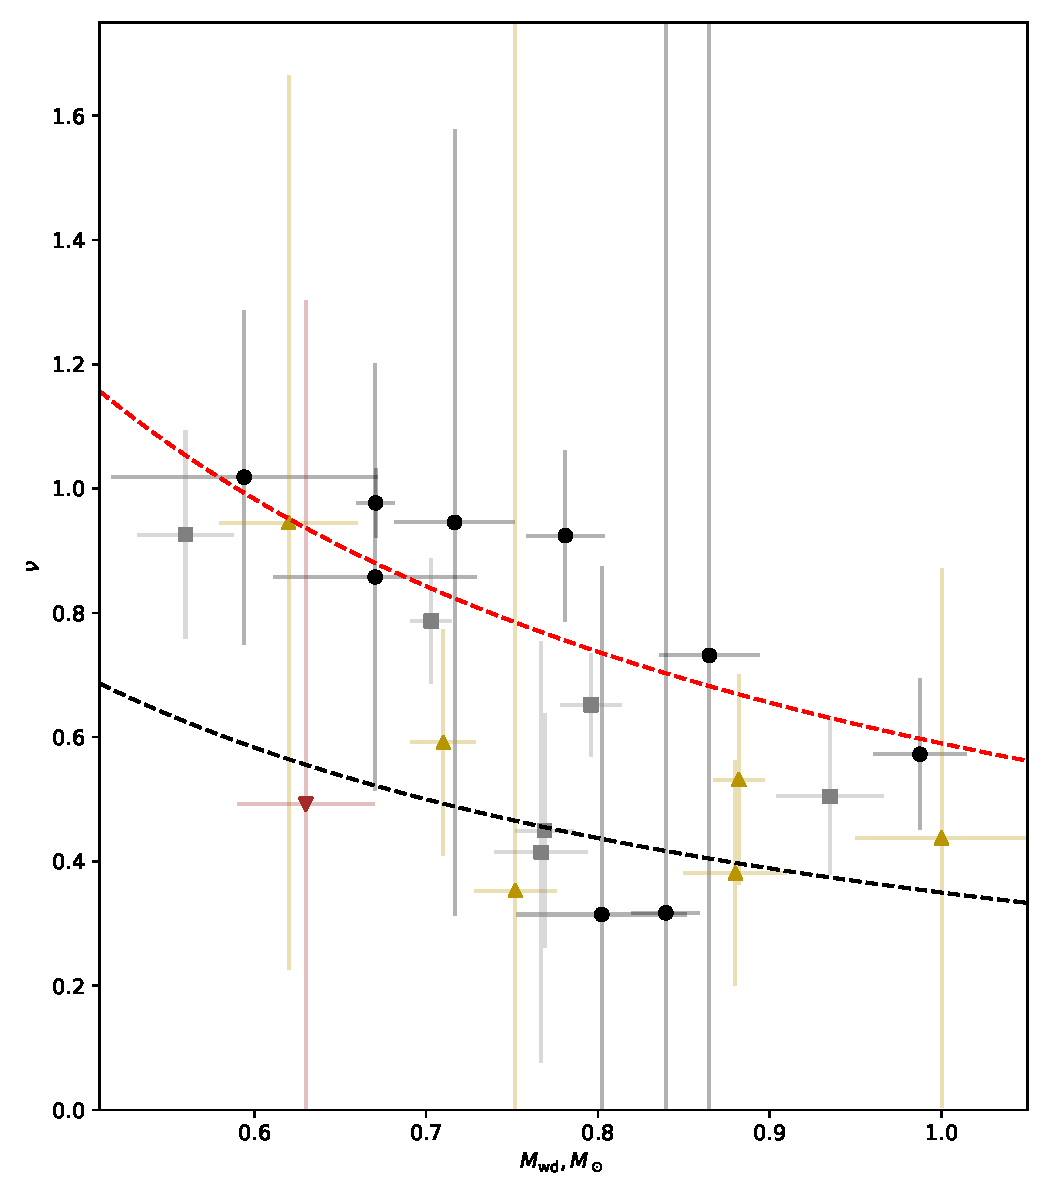
\includegraphics[width=\textwidth]{figures/results/Mdot/nu_for_each_system.pdf}
    \caption{Showing the calculated values of $\nu$ for each short period CV in this sample. Symbols are as in Figure~\ref{fig:massloss and AML:white dwarf mass vs Mdot fit}, though note that for clarity the error bars here are partially transparent. The {\bf dashed black line} shows the eCAML prescription for $\nu = 0.35 / M_{\rm wd}$.}
    \label{fig:massloss and AML:calculated nu for all short period CVs}
\end{figure}



\section{Summary}

I demonstrate the effectiveness of MESA in modelling CV evolution, and produce a configuration that reasonably closely replicates the canonical CV donor evolution. However, I note that with some additional work, MESA should be capable of even closer agreement.
Instead, I focus on exactly reproducing the observed M dwarf mass-radius relationship of \citet{brown2022} by introducing star spots to MESA.
Using these M dwarf models, I infer the mass loss rates of the M dwarf donors of eclipse modelled CVs, by comparing their measured masses and radii with those of MESA models with varying degrees of mass loss.

The results here are considered preliminary for a few reasons. Primarily, the mass-radius relationship used to calibrate the MESA model radii at zero mass loss is incomplete, reverting to theoretical models at $0.121 M_\odot$ -- the majority of my data lie in this poorly understood mass range.
Significant further work is needed to grow the population of eclipse modelled low-$M_{\rm donor}$ CVs and improve these statistics, and continued eclipse modelling targeting short period CVs will be invaluable to confidently determining the source of excess AML.
Specific effort should be targeted towards confident characterisation of CVs at slightly higher $M_{\rm donor}$ of $\sim0.15$ (i.e. a period of $\sim 1.8 - 2.2$ hours), where existing data are somewhat sparse and have large error bars. The clustering of confident data at lower masses leaves the current sample prone to poor sensitivity to data beyond $\sim 0.12 M_\odot$.

Preliminary results suggest that magnetic braking is a poor description of the excess AML inferred from eclipse modelling of CVs, and indicate that eCAML continues to be a better descriptor of the data.
The basic prediction of eCAML -- that the relationship between $\dot J / J$ and $\dot M / (M_{\rm donor} M_{\rm wd})$ is a straight line -- is seen in the data, though I suggest in \S\ref{sect:massloss and AML:systematic bias} that my $\dot M$ are systematically over-estimated.
It must be reiterated, however, that the data presented here are themselves \textit{not} well-described by eCAML.
 Calibrating the eCAML free parameter from these data results in a higher constant of proportionality and concludes that virtually all CVs are dynamically unstable, which is not self-consistent. This is likely a result of the systematic over-estimation of $\dot M$.

